\subsubsection{Sectors Operations}
\label{sec:osg_sectors_ops}  

How to define sectors attributes is defined in \nameref{sec:ui_configure_sectors}. \\

For each defined sector, a colored polygon is shown, grouped by it's layer. Such a structure could look as follows:

\begin{itemize}
 \item Layer A
 \begin{itemize}
 \item Sector A1
 \item Sector A2
\end{itemize} 
 \item Layer B
  \begin{itemize}
 \item Sector B1
\end{itemize} 
\end{itemize}

Each layer or sector can be shown/hidden. The sectors layer display configuration is stored in the configuration and restored upon startup. \\

For the examples shown in the respective task, the following display can be shown:

\begin{figure}[H]
    \hspace*{-2.5cm}
    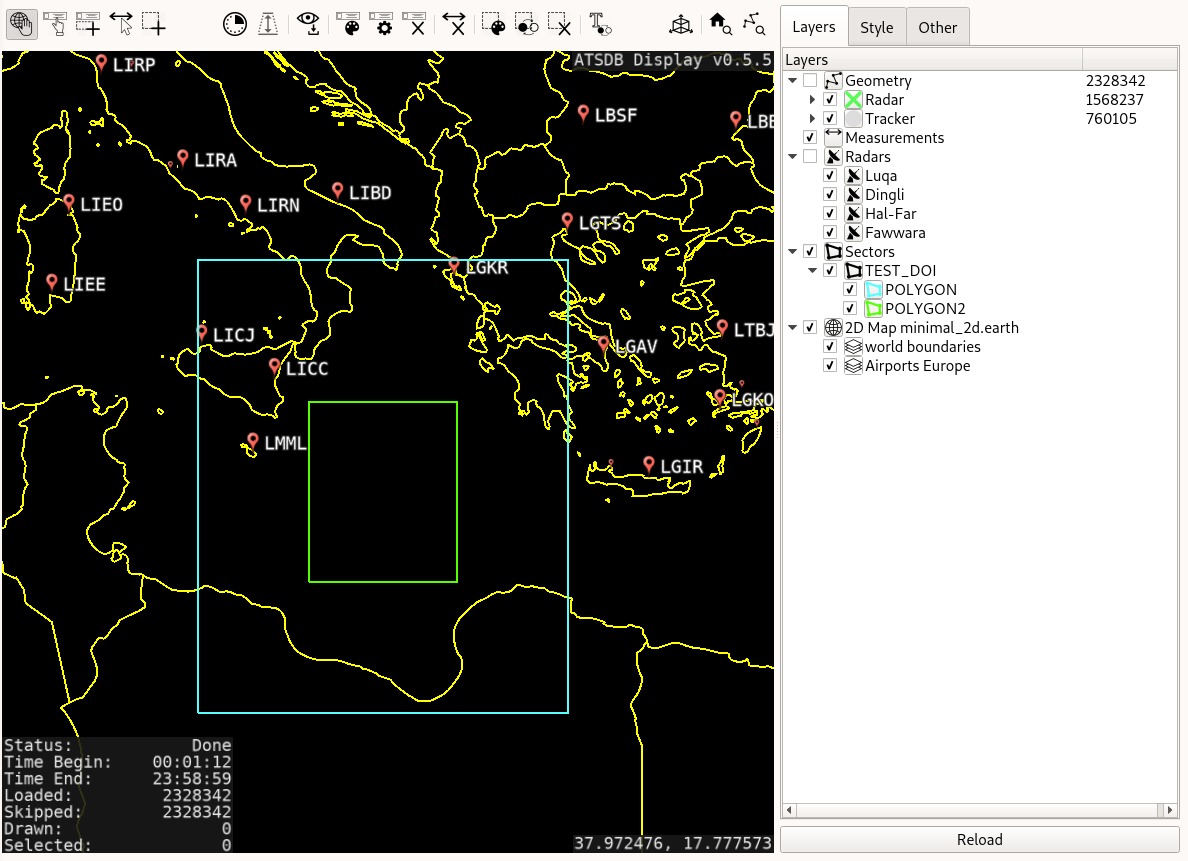
\includegraphics[width=19cm]{figures/osgview_sectors2d.png}
  \caption{OSG View with 2D Sector Examples}
\end{figure}

\begin{figure}[H]
    \hspace*{-2.5cm}
    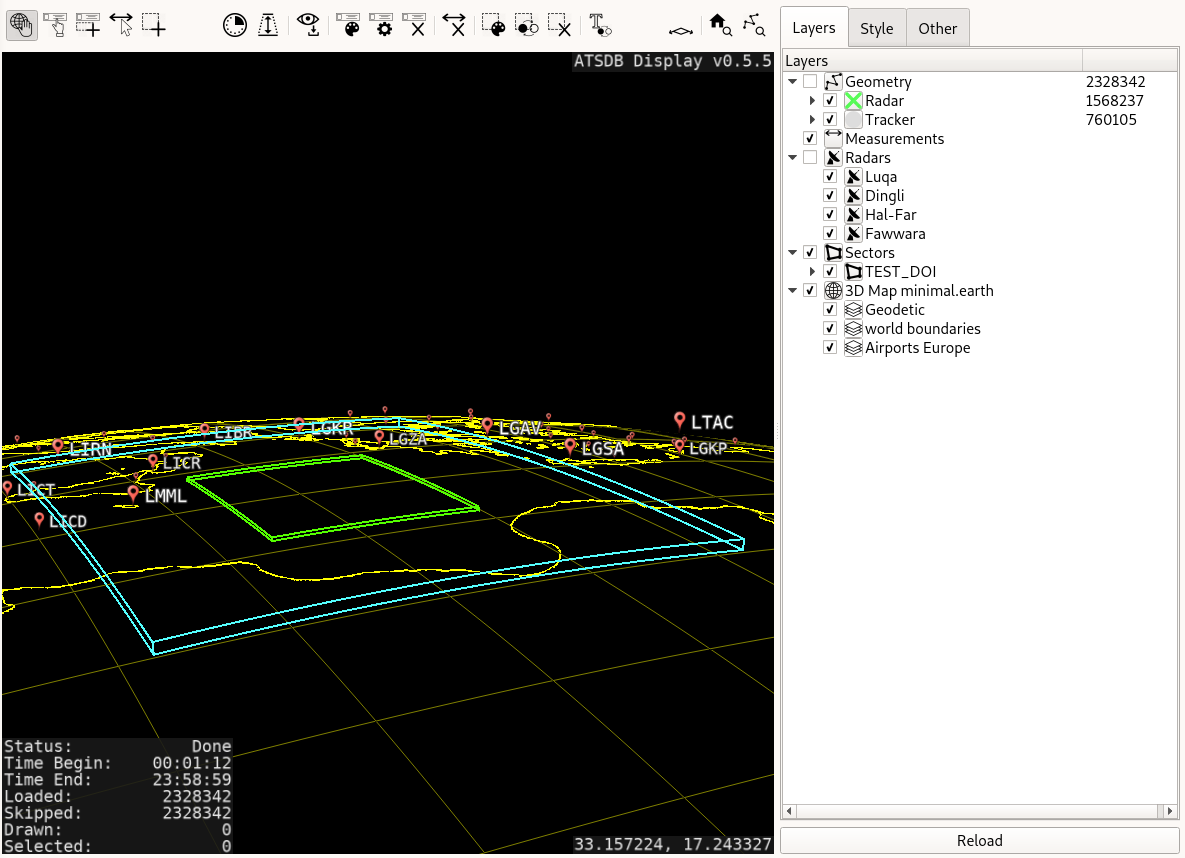
\includegraphics[width=19cm]{figures/osgview_sectors3d.png}
  \caption{OSG View with 3D Sector Examples}
\end{figure}
